% Cours détaillé — Autoencodeurs et débruitage d'images (DAE)
% Document "cours" (texte continu + définitions + formules), distinct de notes_presentateur.tex
% Compilation (dans /docs): pdflatex -interaction=nonstopmode -halt-on-error cours_autoencodeurs_debruitage.tex

\documentclass[11pt,a4paper]{article}

\usepackage[T1]{fontenc}
\usepackage[utf8]{inputenc}
\usepackage[french]{babel}

\usepackage{amsmath,amssymb,mathtools}
\usepackage{geometry}
\geometry{margin=2.4cm}

\usepackage{graphicx}
\usepackage{xcolor}
\usepackage{booktabs}

\usepackage{xurl}
\usepackage{hyperref}
\hypersetup{colorlinks=true, linkcolor=blue!50!black, urlcolor=blue!50!black, citecolor=blue!50!black}
\urlstyle{same}

\usepackage{enumitem}
\setlist[itemize]{leftmargin=1.2em}
\setlist[enumerate]{leftmargin=1.2em}

% Chemins d'images (depuis /docs)
\graphicspath{{../assets/figures/}{../assets/logos/}}

% --- Macros ---
\newcommand{\R}{\mathbb{R}}
\newcommand{\E}{\mathbb{E}}
\newcommand{\norm}[1]{\left\lVert #1 \right\rVert}
\newcommand{\MSE}{\mathrm{MSE}}
\newcommand{\PSNR}{\mathrm{PSNR}}

\title{Cours détaillé : Autoencodeurs et débruitage d'images\\(Denoising Autoencoders)}
\author{Alban Komla Henovi \and Asta Walo Diop \and Arthur Bomemo Walé}
\date{19 avril 2026}

\begin{document}
\maketitle

\begin{abstract}
Ce document est un \textbf{cours} (texte continu) qui accompagne les slides de l'exposé : il explique les autoencodeurs (AE), l'autoencodeur débruiteur (DAE), les modèles de bruit, les architectures convolutionnelles et les métriques (MSE, PSNR, SSIM). Une partie décrit la logique de la démonstration notebook (image locale + patchs) et les points d'attention.
\end{abstract}

\tableofcontents

% -----------------------------------------------------------------------------
\section{Contexte : pourquoi débruiter des images ?}

En imagerie optique (satellite, aérienne, microscopie, photo), les images contiennent du bruit dû à plusieurs facteurs :
\begin{itemize}
  \item bruit électronique du capteur et du système d'acquisition,
  \item conditions d'éclairage et atmosphère,
  \item compression, transmission, prétraitements,
  \item limitations matérielles (ISO élevé, temps d'exposition court, etc.).
\end{itemize}

L'objectif du débruitage est de produire une estimation \emph{plus propre} d'une image à partir d'une observation bruitée.
On peut exprimer cela comme l'apprentissage d'un opérateur paramétré $f_\theta$ (un réseau de neurones) :
\begin{equation}
  x_{\text{clean}} \approx f_\theta(\tilde{x}),
\end{equation}
avec $\tilde{x}$ l'image bruitée et $x_{\text{clean}}$ l'image cible (référence).

\paragraph{Pourquoi l'apprentissage profond ?}
Les méthodes classiques (filtre médian, filtre gaussien, BM3D, etc.) reposent sur des hypothèses explicites sur le bruit et/ou l'image. Les réseaux de neurones permettent d'apprendre une transformation plus riche, guidée par des données.

% -----------------------------------------------------------------------------
\section{Notations et prérequis}

On considère des images normalisées dans $[0,1]$.
\begin{itemize}
  \item $x$ : image \textbf{propre}. Souvent $x \in [0,1]^{H\times W\times C}$.
  \item $\tilde{x}$ : image \textbf{bruitée} construite à partir de $x$.
  \item $\hat{x}$ : image reconstruite / prédite par le modèle.
  \item $\theta$ : paramètres du modèle (poids et biais).
  \item $\ell(x,\hat{x})$ : perte entre une cible et une prédiction.
  \item $m$ : nombre d'exemples sur lesquels on moyenne la perte (taille du dataset ou du mini-batch).
\end{itemize}

Dans la pratique, l'optimisation se fait par mini-batch : on calcule une estimation de la perte sur un petit ensemble (ex. 32) puis on met à jour $\theta$.

% -----------------------------------------------------------------------------
\section{Autoencodeur (AE) : principe}

\subsection{Définition}

Un \textbf{autoencodeur} est composé de deux fonctions paramétrées :
\begin{itemize}
  \item un \textbf{encodeur} $E_\theta$ qui transforme l'entrée $x$ en une représentation latente $z$,
  \item un \textbf{décodeur} $D_\theta$ qui reconstruit une image $\hat{x}$ à partir de $z$.
\end{itemize}

Formellement :
\begin{align}
  z &= E_\theta(x), \quad z \in \R^d, \\
  \hat{x} &= D_\theta(z) = D_\theta\big(E_\theta(x)\big).
\end{align}

\paragraph{Intuition du goulot d'étranglement (bottleneck).}
Si la dimension latente $d$ est trop grande et le réseau trop puissant, il peut apprendre une reconstruction triviale (quasi-identité) sans apprendre de structure intéressante.
Un bottleneck (ou d'autres contraintes : régularisation, bruit, sparsité) force le réseau à extraire l'information la plus utile.

\subsection{Objectif d'entraînement (perte de reconstruction)}

On entraîne un AE en minimisant une perte de reconstruction moyenne :
\begin{equation}
  \mathcal{L}(\theta) = \frac{1}{m}\sum_{j=1}^{m} \ell\big(x^{(j)}, \hat{x}^{(j)}\big).
\end{equation}

Le rôle de $m$ :
\begin{itemize}
  \item si on somme sur tout le dataset : $m$ = nombre total d'exemples,
  \item si on somme sur un mini-batch : $m$ = taille du mini-batch.
\end{itemize}

\subsection{Exemple de perte : MSE}

Pour des images, la perte la plus simple est la \textbf{MSE} (Mean Squared Error) :
\begin{equation}
  \ell(x,\hat{x}) = \frac{1}{N} \norm{x-\hat{x}}_2^2,
\end{equation}
avec $N = H\times W\times C$ le nombre de valeurs (pixels $\times$ canaux).

\paragraph{Interprétation.}
La MSE pénalise fortement les grosses erreurs et favorise une reconstruction « en moyenne ».
Elle est très pratique (différentiable, stable) mais peut conduire à des reconstructions légèrement trop lisses.

\subsection{Schémas}

\begin{center}
\IfFileExists{autoencoder.png}{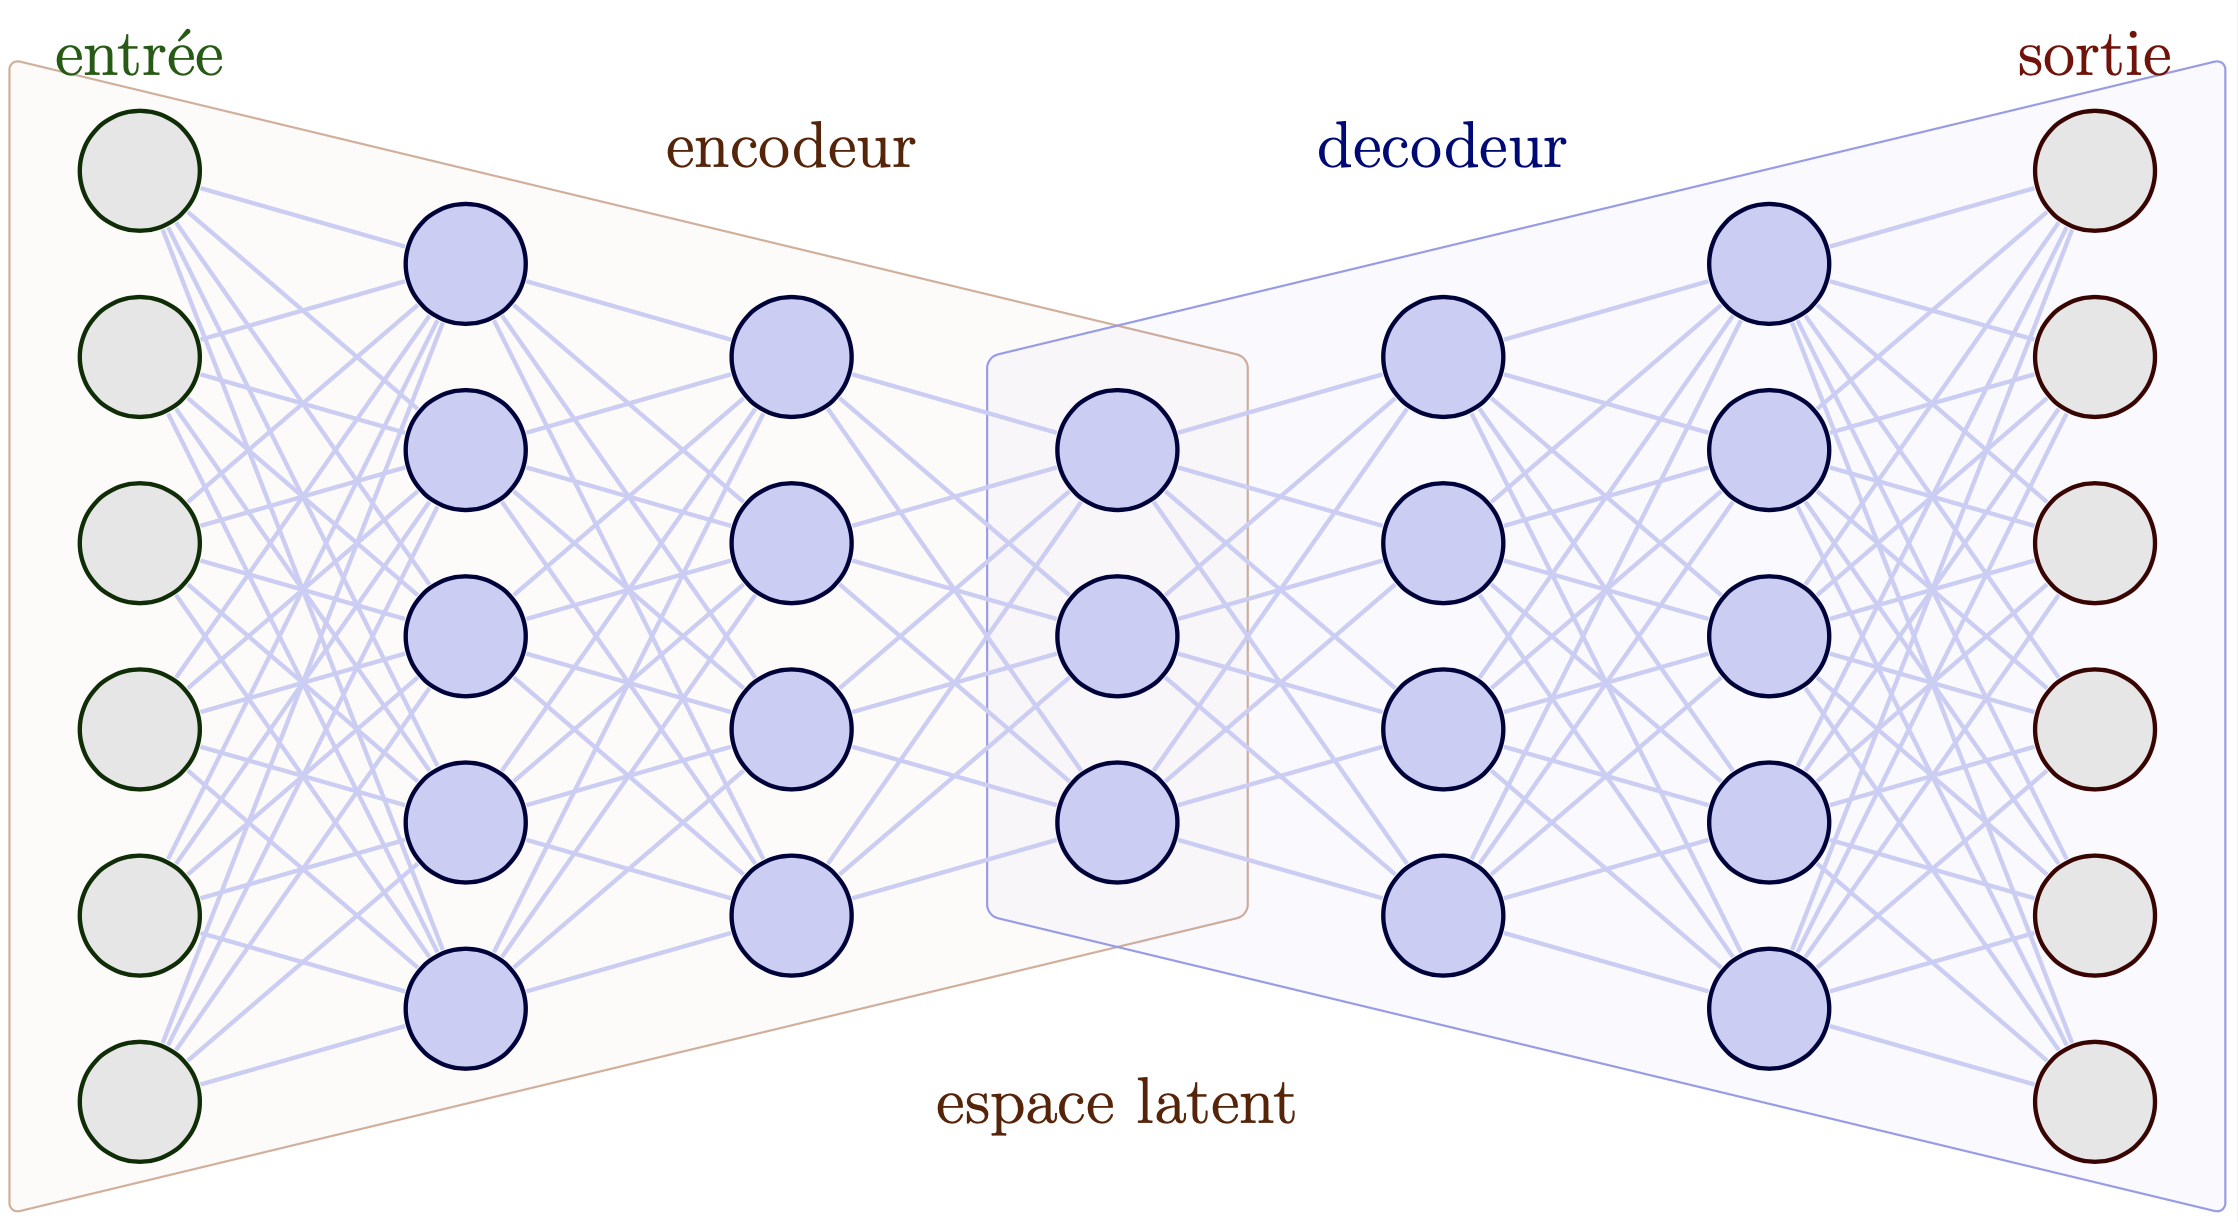
\includegraphics[width=0.92\linewidth]{autoencoder.png}}{\fbox{\parbox{0.92\linewidth}{\centering \small autoencoder.png (absent)}}}
\end{center}

% -----------------------------------------------------------------------------
\section{Autoencodeur débruiteur (DAE)}

\subsection{Idée générale}

L'autoencodeur débruiteur est une variante où l'entrée est volontairement \textbf{corrompue}.
On apprend alors à reconstruire l'image propre $x$ à partir de son observation bruitée $\tilde{x}$.

\begin{center}
\IfFileExists{autoencoder-denoising.png}{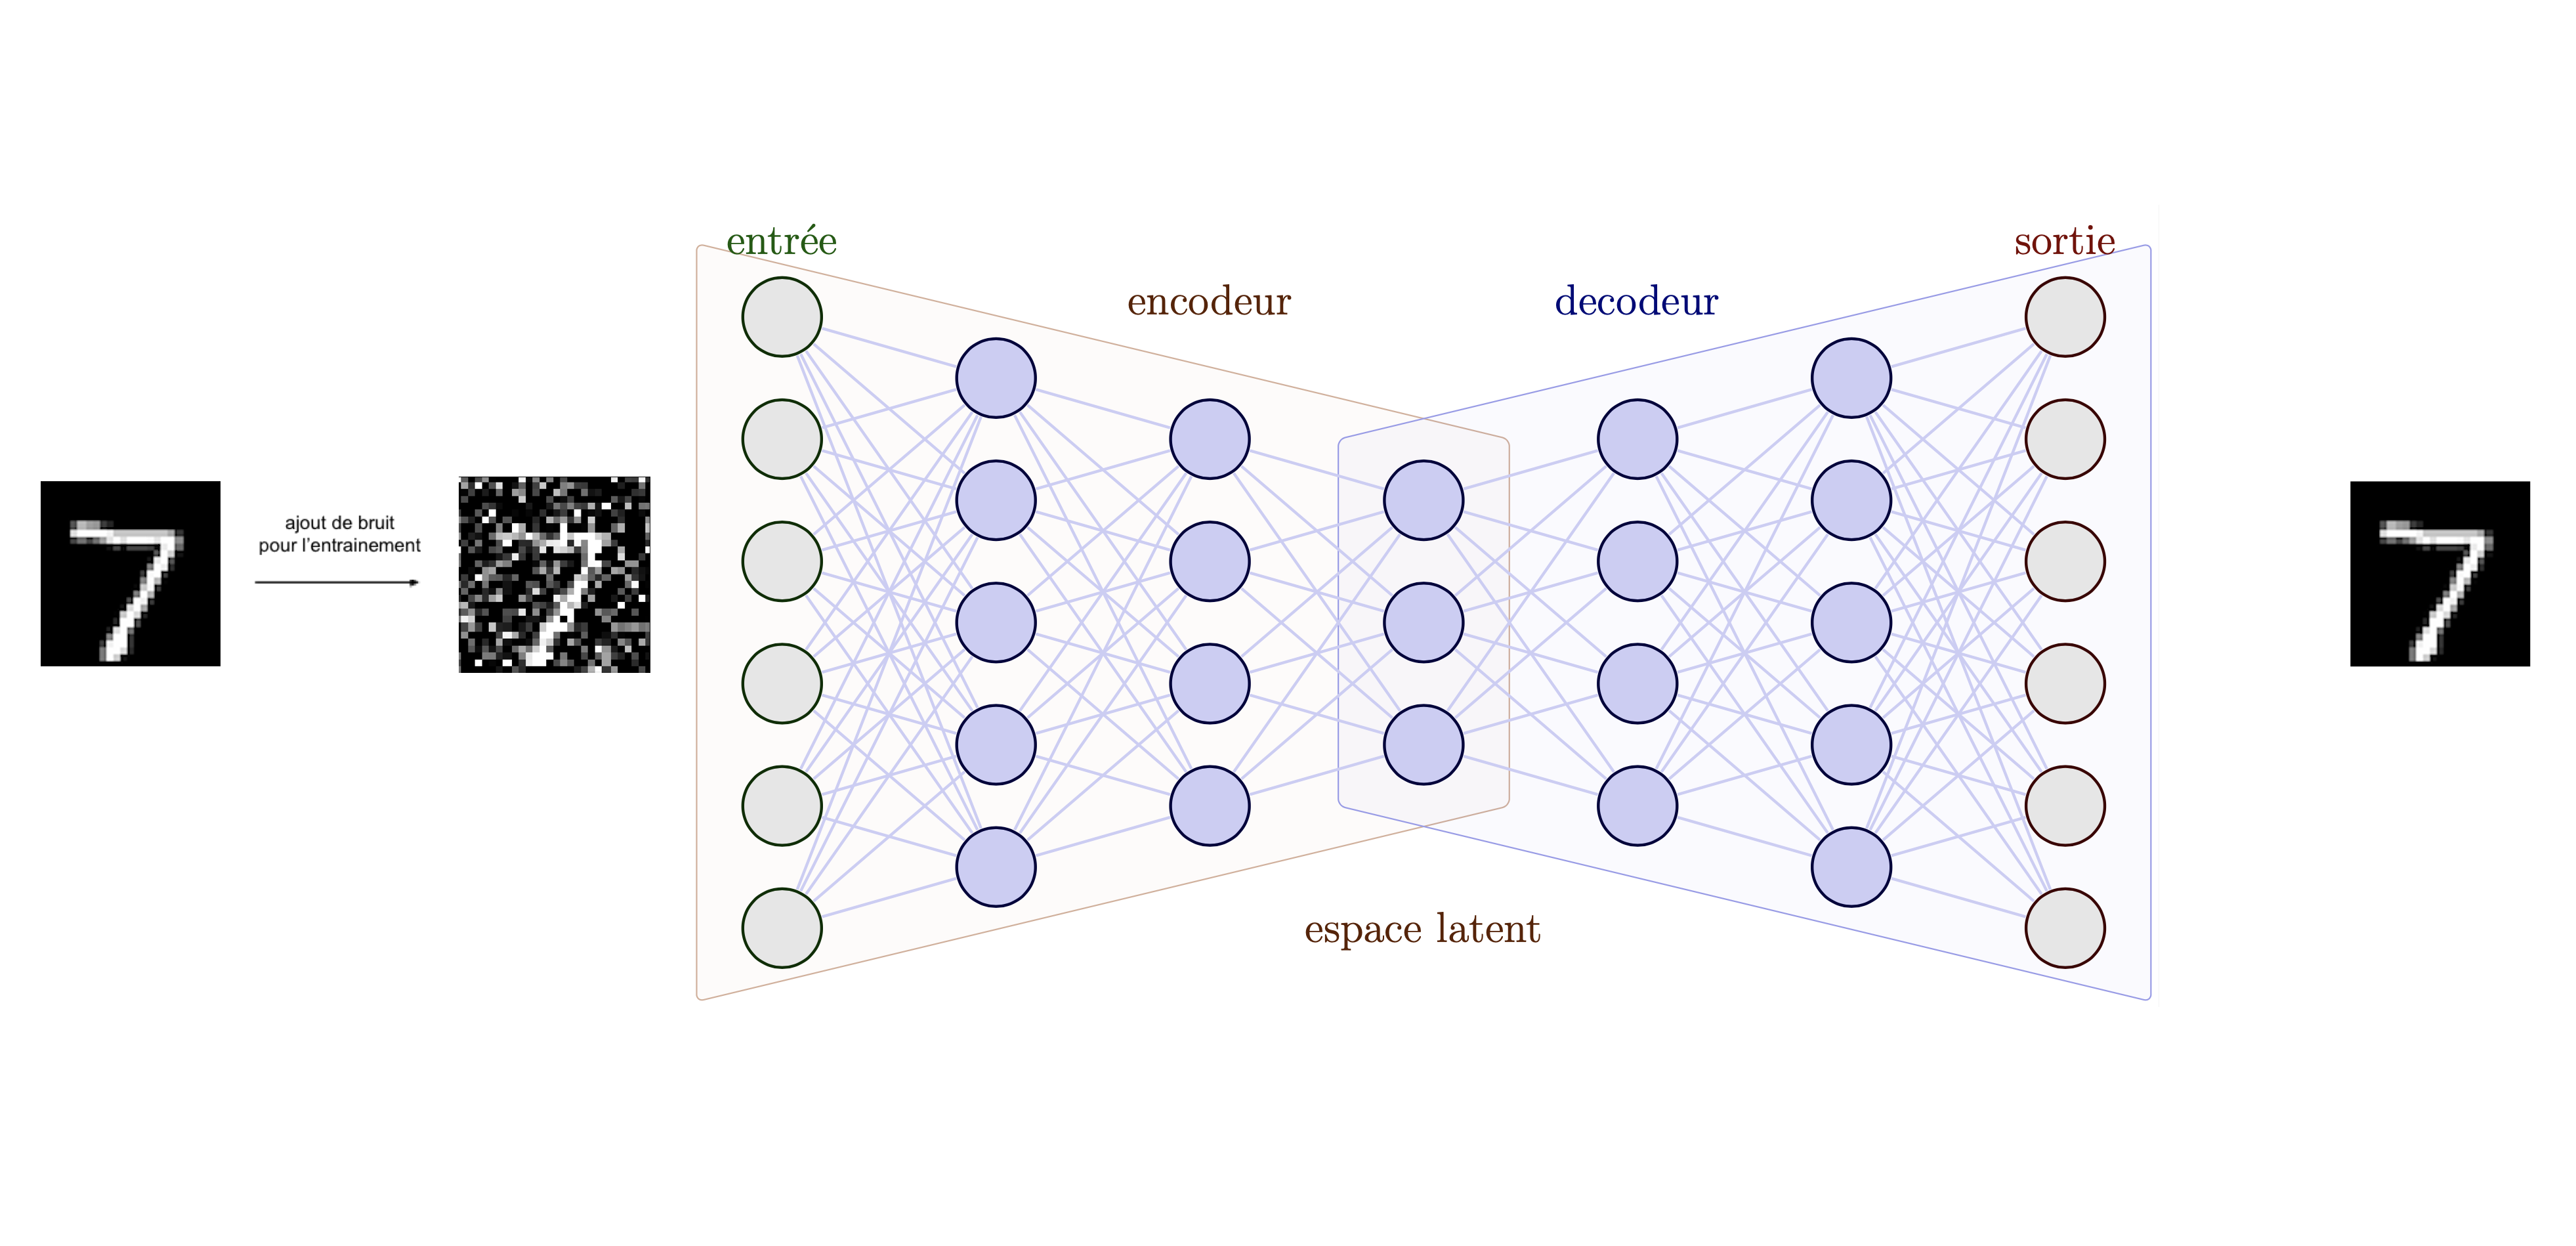
\includegraphics[width=0.92\linewidth]{autoencoder-denoising.png}}{\fbox{\parbox{0.92\linewidth}{\centering \small autoencoder-denoising.png (absent)}}}
\end{center}

\subsection{Formulation probabiliste}

On note $p_{\text{data}}$ la distribution des images propres, et $q(\tilde{x}\mid x)$ la distribution du bruit (le mécanisme de corruption).
L'objectif d'entraînement d'un DAE s'écrit :
\begin{equation}
  \min_{\theta}\; \E_{x\sim p_{\text{data}}}\; \E_{\tilde{x}\sim q(\cdot\mid x)}\; \ell\big(x,\, D_\theta(E_\theta(\tilde{x}))\big).
\end{equation}

\paragraph{Que signifie cette formule ?}
\begin{itemize}
  \item On tire d'abord une image propre $x$ selon les données.
  \item On génère une version bruitée $\tilde{x}$ selon un modèle de bruit.
  \item On fait passer $\tilde{x}$ dans le réseau, on obtient une prédiction $\hat{x}$.
  \item On compare $\hat{x}$ à $x$ avec une perte $\ell$.
  \item On cherche $\theta$ minimisant la perte moyenne.
\end{itemize}

\paragraph{Point crucial.}
Le DAE apprend à retirer \emph{le type de bruit} qu'on lui montre à l'entraînement.
Si le bruit réel est très différent, la performance peut chuter.

% -----------------------------------------------------------------------------
\section{Modèles de bruit (exemples)}

\subsection{Bruit gaussien additif}

Un modèle simple et courant est le bruit gaussien additif :
\begin{equation}
  \tilde{x} = x + \sigma\,\varepsilon,\quad \varepsilon\sim\mathcal{N}(0,I).
\end{equation}

\begin{itemize}
  \item $\varepsilon$ est un bruit aléatoire centré (moyenne nulle).
  \item $\sigma$ contrôle l'intensité du bruit.
  \item On applique souvent un \emph{clipping} pour rester dans $[0,1]$.
\end{itemize}

\subsection{Bruit impulsionnel (sel et poivre)}

On remplace un pourcentage de pixels par 0 ou 1.
Cela simule des erreurs ponctuelles fortes (pixels saturés, pertes de transmission).

\subsection{Bruit multiplicatif (speckle)}

Dans certains capteurs, le bruit est multiplié par le signal :
\begin{equation}
  \tilde{x} = x\odot(1+\varepsilon),
\end{equation}
avec $\odot$ une multiplication terme à terme.

% -----------------------------------------------------------------------------
\section{Architecture : autoencodeur convolutionnel}

\subsection{Pourquoi des convolutions ?}

Les images possèdent une structure spatiale locale (bords, textures). Les convolutions exploitent :
\begin{itemize}
  \item le \textbf{partage de poids} (moins de paramètres),
  \item la \textbf{localité} (filtres $3\times 3$, $5\times 5$, etc.),
  \item une meilleure invariance et généralisation sur les images.
\end{itemize}

\subsection{Encodeur / Décodeur}

Un AE convolutionnel suit souvent ce schéma :
\begin{itemize}
  \item \textbf{Encodeur} : Conv + (Pooling ou strides) pour réduire la résolution et augmenter les canaux.
  \item \textbf{Latent} : représentation compacte (peut être un tenseur, pas forcément un vecteur plat).
  \item \textbf{Décodeur} : UpSampling (ou ConvTranspose) + Conv pour remonter la résolution.
\end{itemize}

\paragraph{Pourquoi cela débruite ?}
Le réseau apprend des filtres qui préservent les structures cohérentes (contours, régions) et atténuent les variations aléatoires incohérentes (bruit).

% -----------------------------------------------------------------------------
\section{Entraînement (procédure)}

\subsection{Pipeline DAE}

Pour chaque image propre $x$ :
\begin{enumerate}
  \item Générer $\tilde{x}$ en ajoutant du bruit (ex. gaussien).
  \item Prédire $\hat{x} = D_\theta(E_\theta(\tilde{x}))$.
  \item Calculer $\ell(x,\hat{x})$ (souvent MSE).
  \item Mettre à jour $\theta$ (descente de gradient, Adam).
\end{enumerate}

\subsection{Mini-batches}

Le calcul exact de $\mathcal{L}(\theta)$ sur tout le dataset peut être coûteux.
On utilise une estimation sur un mini-batch de taille $b$ :
\begin{equation}
  \widehat{\mathcal{L}}(\theta) = \frac{1}{b}\sum_{j=1}^{b}\ell\big(x^{(j)},\hat{x}^{(j)}\big).
\end{equation}

% -----------------------------------------------------------------------------
\section{Métriques d'évaluation}

\subsection{MSE}

\begin{equation}
  \MSE(x,\hat{x}) = \frac{1}{N}\sum_{i=1}^{N} (x_i-\hat{x}_i)^2.
\end{equation}

\subsection{PSNR}

Pour des images dans $[0,1]$, $MAX_I=1$ et :
\begin{equation}
  \PSNR(x,\hat{x}) = 10\log_{10}\Big(\frac{MAX_I^2}{\MSE(x,\hat{x})}\Big)=10\log_{10}\Big(\frac{1}{\MSE(x,\hat{x})}\Big).
\end{equation}

\paragraph{Interprétation.}
\begin{itemize}
  \item PSNR élevé = meilleure qualité (erreur plus faible).
  \item Échelle logarithmique : une même variation de PSNR correspond à un facteur multiplicatif sur la MSE.
\end{itemize}

\subsection{SSIM (Structural Similarity)}

SSIM compare la similarité structurelle locale (luminance, contraste, structure).
Il est souvent mieux corrélé à la perception, mais plus complexe.
Dans une démo pédagogique, MSE/PSNR suffisent souvent.

% -----------------------------------------------------------------------------
\section{Démonstration notebook (ce qui est fait dans votre projet)}

\subsection{Deux modes : MNIST et image locale}

\paragraph{MNIST.}
MNIST est un dataset standard de chiffres manuscrits ($28\times 28$, niveaux de gris). On peut facilement :
\begin{itemize}
  \item ajouter du bruit à une image de chiffre,
  \item entraîner un DAE,
  \item visualiser bruité / débruité / propre.
\end{itemize}

\paragraph{Image locale.}
Quand on veut montrer le principe sur une vraie image (ex. \texttt{image1.webp}), on peut ne disposer que d'une seule image.
Pour entraîner un réseau malgré tout, on fabrique un dataset en découpant en \textbf{patchs} : chaque patch devient un exemple.

\subsection{Pourquoi extraire des patchs ?}

Si l'on n'a qu'une image, un apprentissage direct sur l'image entière peut être instable ou insuffisant (trop peu d'exemples).
En découpant une image en plusieurs patchs, on obtient beaucoup d'exemples $\{p^{(j)}\}_{j=1}^{m}$.
On peut alors entraîner en moyenne sur $m$ patchs.

\subsection{Visualisation et exports}

Le notebook exporte les résultats (pour les slides) et affiche aussi les trois images.
\begin{center}
\IfFileExists{demo_noisy.png}{\includegraphics[width=0.32\linewidth]{demo_noisy.png}}{}\hfill
\IfFileExists{demo_denoised.png}{\includegraphics[width=0.32\linewidth]{demo_denoised.png}}{}\hfill
\IfFileExists{demo_clean.png}{\includegraphics[width=0.32\linewidth]{demo_clean.png}}{}
\end{center}

% -----------------------------------------------------------------------------
\section{Limites et extensions (discussion)}

\begin{itemize}
  \item \textbf{Bruit réel} : si le bruit réel diffère du bruit simulé, il faut adapter $q(\tilde{x}\mid x)$.
  \item \textbf{Sur-lissage} : avec MSE, les reconstructions peuvent perdre des détails fins.
  \item \textbf{Données propres inconnues} : si on ne dispose pas d'images propres, d'autres approches existent (Noise2Noise, self-supervised, etc.).
  \item \textbf{Choix d'architecture} : profondeur, nombre de filtres, type d'upsampling influencent la qualité.
\end{itemize}

% -----------------------------------------------------------------------------
\section{Références}

\begin{itemize}
  \item Ichi.pro (FR) : \url{https://ichi.pro/fr/autoencodeurs-de-debruitage-tensorflow-102261356342629}
  \item LaBRI (P. Preuter) : \url{https://www.labri.fr/perso/preuter/dl2025/cours4-dl.html}
  \item Colab / Eyabennessib : \url{https://colab.research.google.com/github/Eyabennessib/Machine-Learning/blob/main/TP7_autoencodeurs_EBN.ipynb/}
  \item Simon Thomine : \url{https://simonthomine.github.io/CoursDeepLearning/fr/04_Autoencodeurs/02_DenoisingAE.html}
  \item DataCamp (FR) : \url{https://www.datacamp.com/fr/tutorial/introduction-to-autoencoders}
  \item NYU DLSP20 (FR) : \url{https://atcold.github.io/NYU-DLSP20/fr/week07/07-3/}
\end{itemize}

\end{document}
